\chapter{绪论}

\section{研究背景与意义}

随着新一代信息技术与先进制造业的深度融合，工业 4.0 和智能制造已成为全球制造业转型升级的核心驱动力。
在这一宏观背景下，工业数字孪生（Industrial Digital Twin）作为实现物理世界与信息世界交互融合的关键使能技术，正受到学术界与工业界的广泛关注。
数字孪生的核心理念在于通过对物理实体构建多维、多时空尺度的高保真虚拟模型，实现物理空间与虚拟空间的精准交互与实时虚实映射（Virtual-Real Mapping）。
在现代工业制造场景中，高质量的虚实映射不仅是实现设备状态实时监控、生产流程视觉化模拟仿真的基础，更是迈向工业元宇宙和全生命周期智能化管理的重要前提。
在这其中，如何高效、高精度地对复杂的工业物理场景进行三维视觉重建与渲染，是决定数字孪生系统“保真度”与“可用性”的关键核心技术。

然而，构建高保真的工业数字孪生三维视觉底座，在技术实现层面仍面临着巨大的挑战。
传统的工业三维场景构建主要依赖于两类方法：一类是基于计算机辅助设计（Computer-Aided Design, CAD）软件的人工建模，
另一类是基于多视角几何（Multi-View Stereo, MVS）和运动恢复结构（Structure from Motion, SfM）的传统三维重建技术。
CAD 建模虽然能够提供极其精确的理想几何结构，但其构建周期长、人力成本高昂，且模型往往过于理想化，难以反映工业设备在实际运行中的真实磨损、环境光影变化以及复杂材质质感，缺乏视觉上的动态真实感。
另一方面，传统摄影测量与三维重建技术在面对真实的工业场景时，往往显得力不从心。工业现场——如机械加工车间、泵房或自动化产线——普遍存在大量的高反光金属表面、弱纹理区域以及精细复杂的机械结构。传统 MVS 算法在处理这些区域时，极易发生特征匹配失败，导致生成的点云数据严重缺失、表面网格（Mesh）破损不堪，根本无法满足工业数字孪生对视觉“高保真”的苛刻要求。

近年来，以神经辐射场（Neural Radiance Fields, NeRF）为代表的隐式神经渲染技术的出现，为三维场景的高质量重建与新视角合成（Novel View Synthesis）带来了革命性的突破。
NeRF 创造性地利用多层感知机（MLP）将连续的三维场景隐式地编码在神经网络的权重之中，通过体渲染（Volume Rendering）技术，能够极其逼真地还原场景的复杂光影与材质细节。
但是，NeRF 在迈向工业落地的过程中遇到了一道难以逾越的算力鸿沟：其基于光线追踪（Ray Marching）的渲染机制需要对空间进行密集的网络采样，导致推理计算量极为庞大。
在常规硬件下，NeRF 的渲染速度通常只有个位数甚至更低的帧率（FPS），这种严重的延迟完全无法支撑工业数字孪生系统对于实时数据交互、设备高频动态映射以及 VR/AR 沉浸式巡检的实时性需求。

为了打破“渲染质量”与“渲染速度”无法兼得的技术僵局，三维高斯溅射（3D Gaussian Splatting, 3DGS）技术于近期横空出世，并迅速成为三维视觉与计算机图形学领域的研究热点。
3DGS 彻底摒弃了 NeRF 庞大的隐式神经网络，创新性地采用各向异性的三维高斯椭球体作为显式的场景表征基元。
它结合球谐函数（Spherical Harmonics, SH）来表达与视角相关的色彩，最后通过高度并行的可微光栅化（Differentiable Rasterization）管线实现画面的极速渲染。
这种全新的显式辐射场架构在保持甚至超越 NeRF 级高保真渲染质量的同时，成功实现了 100 FPS 以上的实时渲染速度（Real-time Rendering）。
3DGS 的出现，为工业数字孪生的高效虚实映射提供了极具潜力的底层技术框架。

% 预留图表位置：工业数字孪生与虚实映射概念及三维重建技术演进示意图
\begin{figure}[!htbp]
    \centering
    % 后期将 "figures/fig1_1_digital_twin.pdf" 替换为您绘制的图片路径
    % 建议绘制包含：物理车间 -> 传感器/图像采集 -> 3DGS重建 -> 孪生大屏渲染交互的完整闭环
    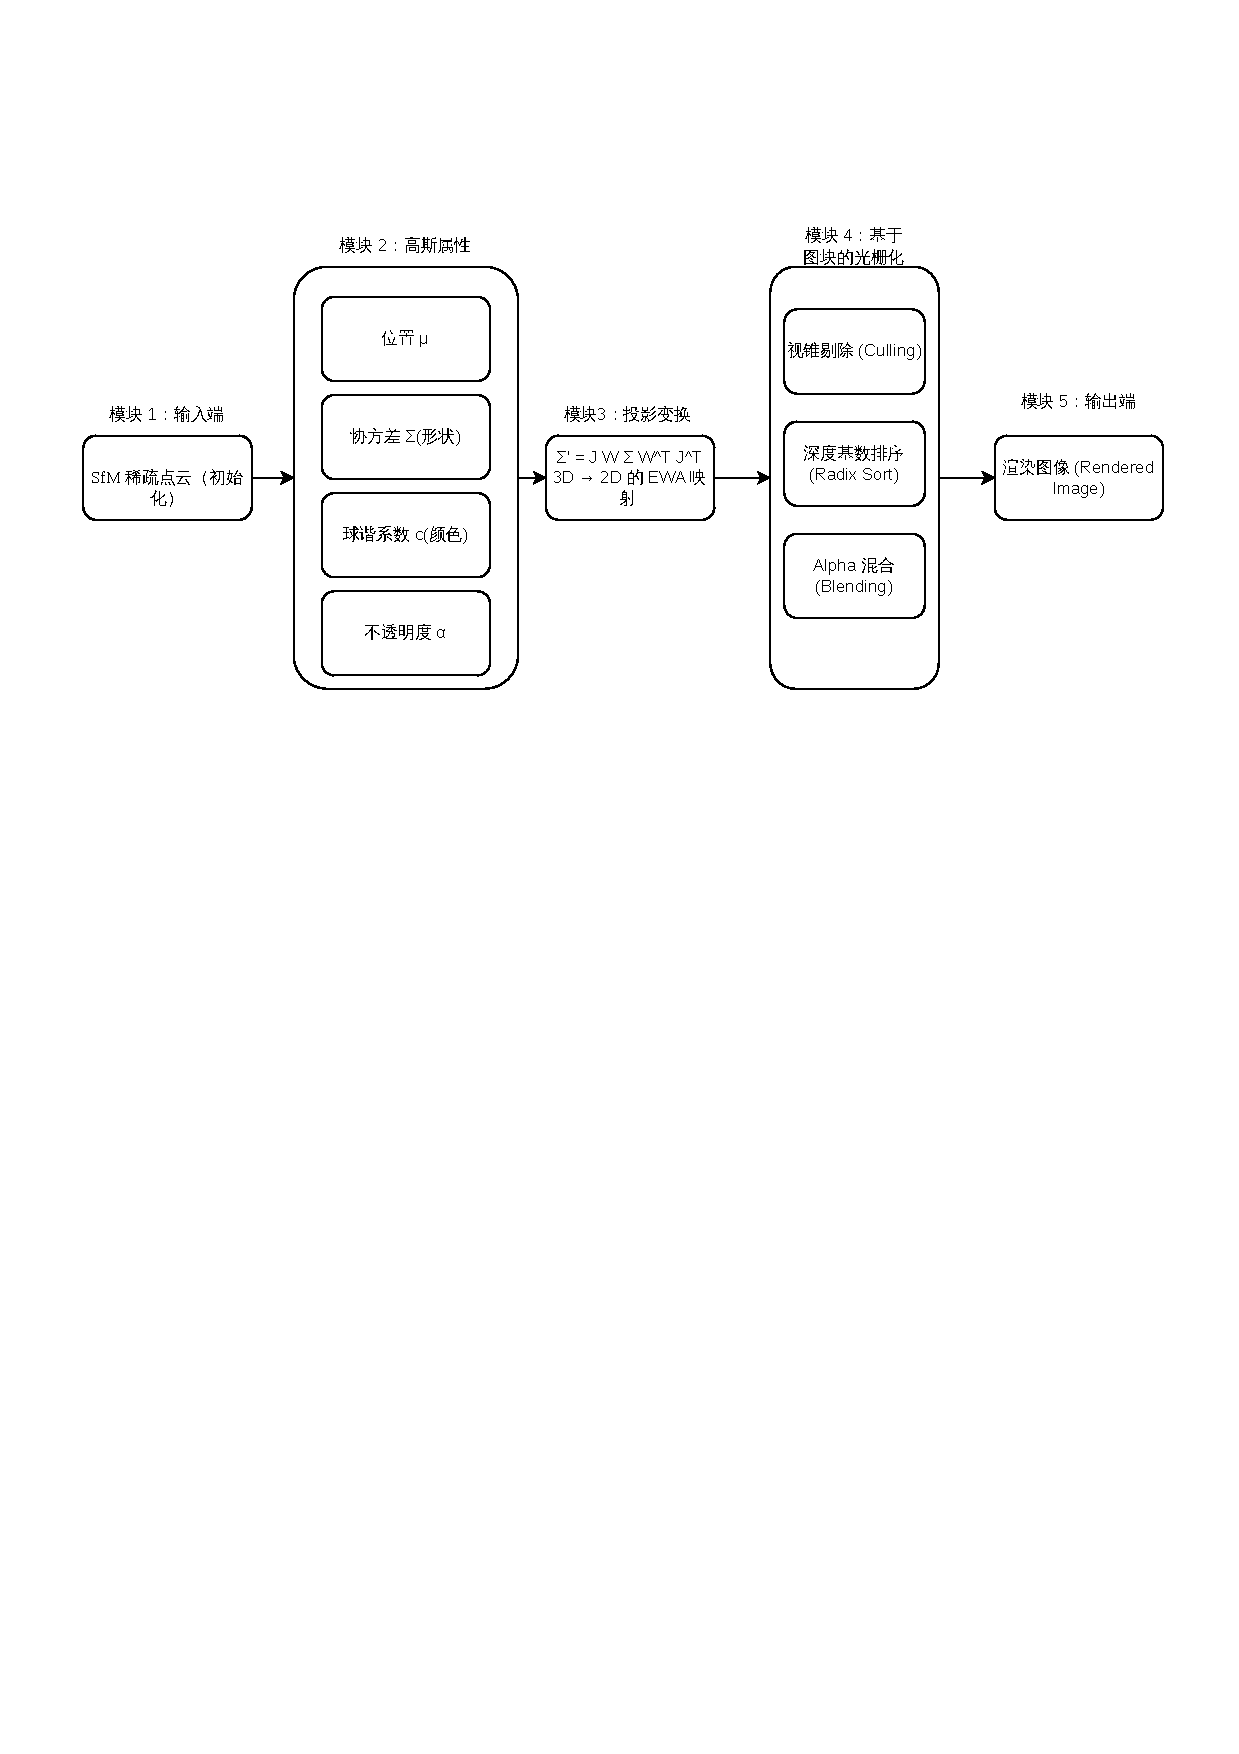
\includegraphics[width=0.85\textwidth, height=0.4\textheight, keepaspectratio]{figures/fig1_1_digital_twin.pdf}
    \caption{面向工业数字孪生的虚实映射架构与三维渲染技术演进示意图}
    \label{fig:digital_twin_concept}
\end{figure}

尽管 3DGS 在实时渲染与高质量表征上展现出了巨大的技术优势，但将其直接应用于大规模、强干扰的工业数字孪生场景时，依然暴露出诸多亟待解决的算法缺陷与工程瓶颈。
首先，3DGS 是一种纯视觉驱动的体辐射表征方法，缺乏对物体表面几何的物理约束。
在面对工业环境中广泛存在的高反光金属材质和弱纹理表面时，原版 3DGS 的优化过程极易陷入局部最优，导致为了拟合局部高光而在半空中生成大量错误的高斯基元，即产生严重的“悬浮物”（Floaters）和多面体视觉伪影，这严重破坏了孪生体的视觉真实度与几何准确性。
其次，3DGS 通过海量的离散高斯基元来拟合场景的精细结构，在表征大规模工业车间或结构极其复杂的重型设备时，高斯点的数量往往呈指数级激增（可达数千万乃至上亿级别）。
这不仅导致模型训练时间过长，更使得存储和渲染时的显存（VRAM）消耗变得极其庞大，对部署设备的显卡算力提出了极为苛刻的要求，严重制约了其在常规设备或边缘计算节点上的规模化应用。

基于上述行业背景与技术痛点，本课题聚焦于工业数字孪生场景下的高保真虚实映射需求，
以 3D 高斯溅射（3DGS）技术为核心研究对象，针对其在工业场景应用中面临的材质泛化性差、几何约束缺失以及显存消耗巨大等瓶颈问题，展开对 3DGS 算法的深度改进与系统化优化研究。
本课题的研究既具有深入的理论探索价值，也具备广泛的工程应用意义。

在理论与算法层面，本研究深入剖析了显式辐射场在复杂光照和反光材质条件下的优化机理。
通过引入单目深度估计与表面法向等多模态几何先验，探索了增强 3DGS 材质解耦与三维空间几何约束的新路径，有效弥补了纯视觉驱动模型在复杂几何表征上的理论盲区；
同时，本研究探索了大规模离散高斯基元的自适应剪枝策略与特征量化方法，为三维显式表示法在大尺度场景下的轻量化、规范化演进提供了新的算法参考，丰富了数字孪生底座模型的三维表征理论体系。

在实际应用层面，本研究的成果能够直击当前工业数字孪生构建过程中“建模难、渲染卡、成本高”的核心痛点。
一方面，通过引入多模态几何约束，显著提升了工业复杂反光设备的重建精度与视觉无伪影表现；
另一方面，通过大幅压缩 3DGS 的显存与存储消耗，使得高保真的“类工业”级三维场景能够在中低端消费级显卡上流畅运行。结合原型系统的融合验证，本研究为制造企业构建低算力门槛、高渲染帧率、高保真度的数字孪生视觉底座提供了一套切实可行的轻量化解决方案，将有力推动虚拟现实交互技术在先进制造业中的落地进程。

\section{国内外研究现状}

\subsection{工业数字孪生与虚实映射技术现状}

工业数字孪生的概念最早可追溯至21世纪初，其核心在于通过数字化手段在虚拟空间中构建物理实体的等价物。
随着工业 4.0 战略的推进，虚实映射技术经历了从静态几何建模向动态高保真视觉表征的演进。
在早期阶段，工业界主要依赖计算机辅助设计（CAD）技术进行三维建模\cite{tao2018digital}。
虽然 CAD 模型在尺寸和几何拓扑上具有绝对的精确性，但其本质是理想化的设计模型，无法反映设备在实际生产车间中的真实物理状态（如磨损、油污、形变），且严重缺乏真实场景的光影与材质质感，导致其在视觉维度的虚实映射存在极强的“塑料感”。

为了获取包含真实纹理的物理世界三维表征，基于多视角几何（Multi-View Stereo, MVS）和运动恢复结构（Structure from Motion, SfM）的摄影测量技术逐渐被引入工业三维重建领域。
以 COLMAP\cite{schonberger2016structure} 为代表的传统三维重建管线，通过特征点提取与匹配、稀疏点云生成以及稠密网格重建，能够从多视角图像中恢复场景的三维结构。
然而，工业生产环境极为复杂，设备表面往往由大面积的弱纹理外壳或高反光金属材质构成。
在这些区域，基于图像局部特征匹配的传统算法极易失效，导致重建出的三维点云存在大量孔洞，生成的表面网格（Mesh）凹凸不平且伴随严重的拓扑错误。
此外，传统管线将场景的光照、材质与几何进行强绑定，一旦视角或环境光发生变化，其渲染结果的保真度便会急剧下降。
因此，探索能够在复杂光照和反光材质下实现高保真视觉表征的新型三维重建技术，成为了工业数字孪生领域亟待突破的瓶颈。

\subsection{神经辐射场 (NeRF) 三维重建进展}

2020年，Mildenhall 等人\cite{mildenhall2020nerf} 首次提出了神经辐射场（Neural Radiance Fields, NeRF），在三维计算机视觉领域引发了范式级的变革。NeRF 利用全连接神经网络（MLP）将连续的三维场景隐式地参数化，输入空间坐标和视角方向，输出对应点的体密度（Volume Density）和辐射度（Color），最终通过可微的体渲染（Volume Rendering）技术合成极其逼真的新视角图像。相比于传统基于离散网格或点云的表征方法，NeRF 展现出了前所未有的视点连续性和极高的照片级真实感，为解决工业复杂材质的视觉表征提供了全新思路。

自 NeRF 提出以来，国内外学者针对其在渲染质量和训练效率上的缺陷进行了大量改进研究。在渲染质量方面，Barron 等人\cite{barron2021mipnerf} 提出了 Mip-NeRF，通过引入圆锥体光线追踪替代传统的单一射线采样，有效解决了多分辨率下场景渲染的混叠（Aliasing）问题；针对强反光表面的重建难题，Ref-NeRF\cite{verbin2022refnerf} 通过引入视角相关的法向量和反射辐射度，大幅改善了模型对镜面反射和光泽表面的拟合效果，这为工业金属材质的重建提供了重要参考。在训练与渲染加速方面，Müller 等人\cite{muller2022instant} 提出了 Instant-NGP，创新性地采用多分辨率哈希网格（Hash Grid）结构替代纯 MLP 网络，将场景的特征存储在可学习的网格节点中，从而将 NeRF 的训练时间从数天缩短至数分钟。

尽管上述改进极大地推动了隐式神经渲染技术的发展，但 NeRF 及其变体依然面临着难以克服的固有缺陷：其核心的体渲染机制依赖于对每条光线进行密集的三维空间采样，每次采样均需查询神经网络或哈希表。这种庞大且密集的计算开销导致其在常规消费级硬件上的推理速度极低。即使是经过深度优化的 Instant-NGP 或 MobileNeRF\cite{chen2023mobilenerf}，在面对 4K 高分辨率或大规模复杂工业场景时，其渲染帧率（FPS）依然难以满足工业数字孪生系统对实时交互、低延迟漫游（如 VR/AR 巡检）的硬性指标。

\subsection{3D高斯溅射 (3DGS) 及其优化研究现状}

为了彻底解决 NeRF 渲染速度慢的痛点，Kerbl 等人\cite{kerbl20233dgs} 于 2023 年提出了三维高斯溅射（3D Gaussian Splatting, 3DGS）技术。与 NeRF 采用隐式连续场不同，3DGS 回归了显式的场景表征范式。它使用数百万个携带位置、协方差矩阵、不透明度和球谐函数（SH）系数的各向异性三维高斯椭球体来拟合场景。在渲染阶段，3DGS 摒弃了耗时的光线追踪，采用高度并行的可微光栅化（Differentiable Rasterization）技术，将三维高斯体投影至二维图像平面进行基于透明度的色彩混合（Alpha Blending）。这种架构在维持高保真视觉质量的同时，实现了百帧以上的实时渲染速度，被视为下一代三维视觉重建的核心底座。

目前，学术界围绕 3DGS 的优化展开了极其热烈的研究，结合工业数字孪生的应用需求，其研究现状主要集中在以下三个主要流派：

\subsubsection{（1）面向复杂材质的几何约束与表面重建优化}
原版 3DGS 是一种纯粹的体表征方法，其高斯基元的空间分布往往呈混沌状态，难以直接提取出精确的物理表面。在工业场景中，面对反光设备时，3DGS 极易通过在相机光心与物体表面之间的空白区域生成高斯点来“欺骗”损失函数，从而产生严重的“悬浮物”（Floaters）。为了解决这一问题，近期涌现了大量基于几何约束的优化研究。Guédon 等人\cite{guedon2024sugar} 提出了 SuGaR，通过在 3DGS 的优化过程中引入正则化项，强制高斯基元对齐到场景的真实表面，从而能够利用泊松重建（Poisson Reconstruction）提取出高质量的表面网格（Mesh）；Huang 等人\cite{huang20242dgs} 提出了 2DGS，将三维的高斯椭球扁平化为二维的椭圆面片（Surfels），从物理直觉上更贴合不透明物体的表面属性，显著提升了多视角的几何一致性。此外，部分研究开始引入多模态先验知识，如利用单目深度估计大模型（如 Depth Anything\cite{yang2024depthanything}）或法向量先验，在损失函数中增加空间结构约束，有效抑制了反光表面的伪影生成。这为本课题第三章面向工业复杂反光材质的自适应几何约束算法提供了直接的理论依据。

\subsubsection{（2）面向大规模场景的轻量化与模型压缩策略}
显存消耗巨大是 3DGS 迈向工业级大场景部署的最大阻碍。原版 3DGS 在表征复杂场景时，往往会生成数千万个高斯点，每个点包含 59 个浮点数参数，导致一个场景的模型体积高达数 GB，渲染显存消耗动辄十几 GB。为此，轻量化（Lightweight）与模型压缩（Compression）成为了另一大研究热点。Lee 等人\cite{lee2024compact3dgs} 提出了 Compact 3DGS，通过引入可学习的掩码（Mask）机制剔除冗余和对视觉贡献极小的高斯基元，并对保留的高斯属性进行量化编码；Fan 等人\cite{fan2024lightgaussian} 的 LightGaussian 则利用全局显著性评估策略，对高斯点云进行自适应剪枝（Pruning），并结合知识蒸馏技术对球谐函数进行降维。另一项突破性工作 Scaffold-GS\cite{lu2024scaffoldgs} 利用稀疏的体素网格（Voxel Grid）作为“脚手架”，将高斯基元的属性锚定在网格特征上，通过多层感知机动态解码，大幅减少了离散高斯基元的绝对数量。这些前沿研究证明了 3DGS 内部存在巨大的参数冗余，为本课题第四章提出针对大规模工业场景的自适应剪枝与特征量化算法奠定了基础。

\subsubsection{（3）渲染质量增强与抗混叠技术}
除了几何与显存优化，进一步提升渲染的保真度和鲁棒性也是学术界关注的重点。在面临不同分辨率或缩放尺度渲染时，原版 3DGS 容易出现锯齿和伪影。为此，Yu 等人\cite{yu2024mipsplatting} 提出了 Mip-Splatting，借鉴 Mip-NeRF 的思想，通过引入二维多尺度滤波器对高斯协方差矩阵进行调制，有效解决了 3DGS 在缩放和平移过程中的高频混叠问题。同时，针对动态工业场景的需求，Dynamic 3DGS 等变体也相继被提出，通过引入时间维度的形变场，使 3DGS 具备了表征非刚性运动物体的能力。

% 预留图表位置：NeRF 与 3DGS 渲染管线对比示意图
\begin{figure}[htbp]
    \centering
    % 后期将 "figures/fig1_2_nerf_vs_3dgs.pdf" 替换为您绘制的图片路径
    \safeimage[\textwidth]{figures/fig1_2_nerf_vs_3dgs.pdf}
    \caption{隐式神经辐射场(NeRF)与显式三维高斯溅射(3DGS)渲染管线对比}
    \label{fig:nerf_vs_3dgs}
\end{figure}

\subsection{现有技术的局限性与挑战}

综上所述，三维视觉重建技术在经历了传统 MVS、NeRF 到 3DGS 的跨越式发展后，已取得了极其显著的进步。
然而，面向工业数字孪生这一高度垂直且条件苛刻的应用场景，现有技术仍存在“水土不服”的局限性。

% 插入表格：主流三维重建算法在工业级场景中的性能对比
\begin{table}[htbp]
    \centering
    \caption{主流三维场景重建与渲染算法综合性能定性对比}
    \label{tab:algorithm_comparison}
    \renewcommand{\arraystretch}{1.4} % 稍微增加行高，防止换行后文字太挤
    \small % 适当缩小字号，更符合学术论文对宽表格的处理
    \setlength{\tabcolsep}{3pt} % 稍微收缩列间距，挤出更多空间
    
    % 使用 tabularx，设置总宽为页面宽度 \textwidth
    % L/C/R 是自定义的自动换行且指定对齐方式的列类型
    \begin{tabularx}{\textwidth}{l l c c >{\centering\arraybackslash}X >{\centering\arraybackslash}X}
        \toprule
        \textbf{算法类型} & \textbf{代表性工作} & \textbf{渲染帧率} & \textbf{显存占用} & \textbf{反光材质} & \textbf{几何表面} \\
         & & \textbf{(FPS)} & & \textbf{鲁棒性} & \textbf{提取} \\
        \midrule
        传统多视角几何 & COLMAP & 无法直接渲染 & 极低 & 极差 & 差（易破损） \\
        隐式神经辐射场 & Mip-NeRF & 极低 ($<1$) & 中等 & 较好 & 较好 \\
        加速隐式辐射场 & Instant-NGP & 中等 ($\sim 15$) & 中等 & 一般 & 一般 \\
        显式高斯溅射 & 原版 3DGS & 极高 ($>100$) & 极高 (爆炸风险) & 较差 (伪影严重) & 极差 \\
        \bottomrule
    \end{tabularx}
\end{table}

结合表 1-1 的对比分析可以看出，现有的大部分改进研究往往呈“单点突破”态势。例如，侧重于表面提取的算法（如 SuGaR）通常会牺牲一定的渲染帧率，并进一步增加优化过程的计算复杂度；而侧重于轻量化压缩的算法（如 Compact 3DGS）虽然降低了显存消耗，但在处理工业高光和弱纹理区域时，由于基元数量锐减，更容易导致视觉质量的崩塌。

在实际的工业虚实映射中，我们面临的痛点往往是复合型的：既要求模型能够高保真地还原反光金属设备（需要强大的多模态几何约束），又要求模型具备足够小的显存占用以支撑整个大尺度车间的实时漫游（需要深度的轻量化压缩）。目前，鲜有研究将这两种优化方向在统一的工业背景下进行深度融合与自适应调优。因此，深入研究一种能够兼顾“高保真（克服复杂材质）”与“高效率（极低显存与高帧率）”的 3DGS 融合优化算法，并将其集成打通至数字孪生验证系统中，正是本课题切入的痛点所在，也是本课题突破现有技术壁垒的核心挑战。


\section{论文的主要工作}

针对当前 3D 高斯溅射（3DGS）技术在应用于工业数字孪生时，面临的复杂反光材质重建精度低、大规模场景显存消耗巨大，以及缺乏系统级验证等核心痛点，本文以实现面向工业场景的高效、高保真虚实映射为最终目标，从空间几何约束增强、场景模型轻量化压缩以及端到端验证系统构建三个递进的维度展开了深入研究。本文的主要研究工作与创新点可以概括为以下三个方面：

\textbf{（1）提出了面向类工业场景的多模态自适应几何约束重建算法}

在工业制造与运维环境中，设备表面往往由大面积的高反光金属、拉丝不锈钢或高光泽喷漆构成，同时伴随大量缺乏纹理细节的平坦外壳。原版 3DGS 作为一种纯视觉驱动的显式体表征方法，在处理这类区域时极易出现多视角几何一致性缺失的问题，导致在三维空间中生成大量用于“欺骗”损失函数的冗余悬浮物（Floaters）和多面体伪影，严重破坏了虚实映射的真实感。

针对上述问题，本文提出了一种融合多模态几何先验的自适应 3DGS 重建算法。首先，在传统的多视角 RGB 图像序列基础之上，本文引入了强大的单目深度估计大模型（如 Depth Anything\cite{yang2024depthanything}）作为多模态信息的补充，提取场景的稠密深度图先验；其次，在 3DGS 的可微光栅化管线与优化框架中，设计并引入了深度的像素级一致性损失（Depth Consistency Loss）与基于局部平滑假设的表面法向正则化项（Normal Regularization）；最后，提出了一种自适应的权重动态调节机制，使模型在优化初期依赖几何先验收敛整体结构，在优化后期依赖色彩损失恢复高频细节。实验表明，该算法有效抑制了复杂反光材质表面的视觉伪影，强制高斯基元贴合真实的物理表面，不仅显著提升了新视角合成的图像保真度，更为后续提取精确的工业设备三维表面网格（Mesh）奠定了坚实的几何基础。

\textbf{（2）提出了面向大规模工业孪生场景的 3DGS 轻量化表达与压缩算法}

工业数字孪生往往需要对大尺度、极其复杂的生产车间或重型装备进行全景级的三维表征。原版 3DGS 在此类场景下会自适应生长出数千万乃至上亿个携带大量高维参数（如球谐函数系数、三维协方差矩阵等）的高斯基元。这不仅导致模型存储文件极其臃肿，更在实时渲染时消耗惊人的显存（VRAM），使得高保真虚实映射难以在企业中低端消费级计算节点或边缘设备上普及。

为突破这一算力瓶颈，本文提出了一套针对工业大场景的 3DGS 自适应轻量化与参数压缩算法框架。该框架首先通过建立高斯基元的“视觉显著性与几何贡献度”综合评估模型，对场景中的离散高斯点进行重要性排序；在此基础上，设计了一种空间自适应的非对称剪枝策略（Adaptive Pruning），在保证边缘高频细节不丢失的前提下，大幅剔除重叠冗余、低透明度以及位于平坦内部区域的无效高斯点；随后，针对保留下来的有效高斯基元，引入特征向量量化（Vector Quantization）与低秩近似技术，对占据极高显存的球谐函数（SH）系数进行降维压缩编码。该工作在几乎不降低渲染质量（PSNR、SSIM 等指标）的前提下，将场景模型的参数量与显存消耗压缩了数量级，成功打破了大规模场景渲染的硬件限制。

\textbf{（3）构建了基于融合改进 3DGS 的高保真验证系统与综合实验评估}

为了充分验证上述前沿算法在实际类工业应用场景中的可行性与优越性，避免研究仅停留在单一理论层面，本文将“多模态自适应几何约束”与“轻量化表达压缩”两种算法在代码与管线层面进行了深度联合调优，构建了一套端到端的轻量级虚实映射算法原型验证系统。

考虑到真实工业封闭车间的数据获取壁垒，本文在实验验证环节设计了“标准开源数据与自采类工业数据”相结合的综合评估策略。
一方面，利用具有广泛学术认可度的 Tanks and Temples\cite{} 与 DTU\cite{} 等包含复杂几何与大型人造物体的开源数据集进行基准测试；
另一方面，在校园工训中心与后勤设施中，专门采集了包含复杂机械臂、强反光管道箱体等设备的“自采类工业场景多视角数据集”。
通过搭建的验证系统，将本文的融合算法与传统 NeRF 及原版 3DGS 进行了全面的消融实验与横向对比。
结果不仅在客观评价指标（如渲染帧率 FPS、显存占用量、峰值信噪比等）上证明了本文方法的综合领先性，更通过交互式三维可视化工具（Viewer）直观展示了其在常规显卡下实现高帧率、无伪影漫游的能力，
验证了其落地赋能智能制造三维底座的巨大潜力。

% 插入图表：图1-3 本文研究内容技术路线图
\begin{figure}[htbp]
    \centering
    % 请在后期将 "figures/fig1_3_tech_route.pdf" 替换为你实际绘制的图片路径
    % 建议使用 Visio 或 draw.io 绘制流程图：从输入数据 -> 深度/法向约束模块 -> 剪枝/压缩模块 -> 融合系统 -> 验证输出
    \safeimage[\textwidth]{figures/fig1_3_tech_route.pdf}
    \caption{本文主要研究内容与技术路线图}
    \label{fig:tech_route}
\end{figure}